\begin{figure}
\centering
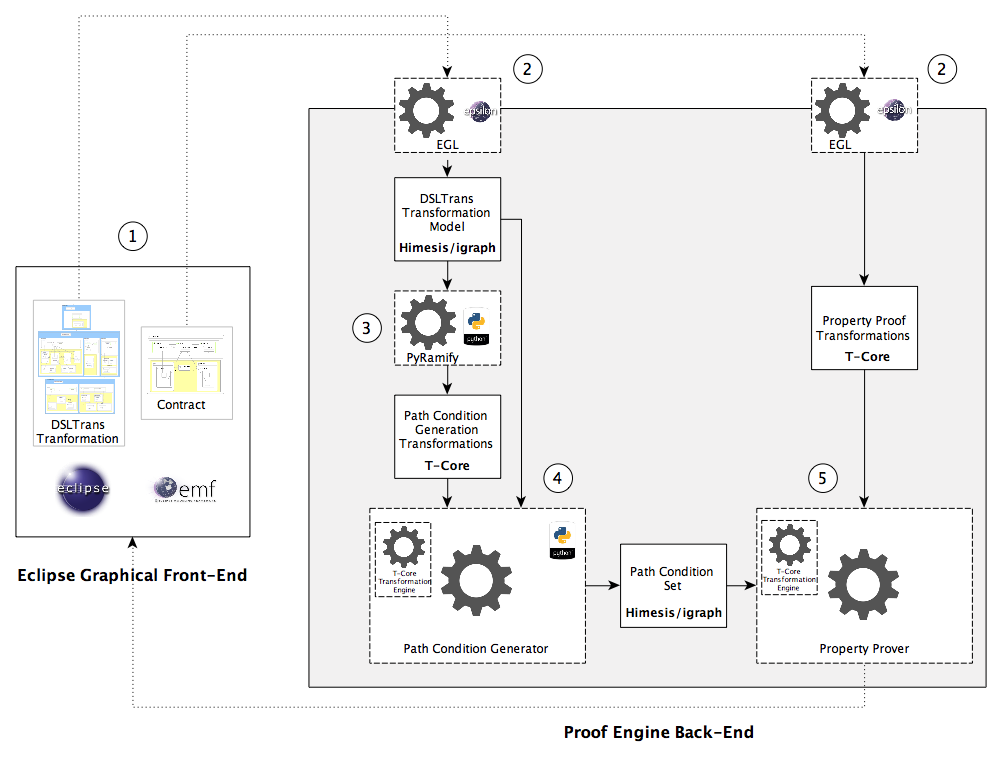
\includegraphics[width=0.45\textwidth]{figures/syvolt_arch}
\caption{The architecture of the SyVOLT tool}
\label{fig:arch}
\end{figure}

Figure~\ref{fig:arch} shows the architecture of the SyVOLT tool. We will now briefly visit each component in turn, mentioning the main technologies and languages employed.


One principle of the Modelling, Design, and Simulation Lab is that all tools and processes should be explicitly modelled at an appropriate abstraction level. The next section will describe how we have applied this practice 

Everything is modelled. Model transformations, and tooling.

Everything is a model or a transformation.



An Ant[CITE] script is then run from within the Eclipse environment. This script will orchestrate the following components.


\subsection{Generating Artifacts}
For our contract prover, there are a number of artifacts that need to be generated. For example, typed graphs (in the Himesis format[CITE]) are generated from each rule and contract, using the Eclipse Generation Language (EGL). As well, the top-level Python scripts used to prove contracts are also generated through this method.

This use of EGL allows for precise control over the artifacts that are produced, while taking a relatively short amount of time to create and debug.
Model-to-text generation.



\subsection{PyRamify}

PyRamify is a Python script that takes as input Himesis graphs representing the rules in the transformation. Then, through the RAMification procedure [CITE RAM], matchers for each rule are produced. These matchers will then match over the rules, which allows the contract prover to determine how rules might execute over an input model. Rewriters are also produced with traceability information, which will properly apply the right-hand side of a rule when it matches.

Currently, PyRamify is implemented as a Python script, as we were unable to implement automatic creation of higher-order artifacts in another modelling tool. We could not find technology to do higher-higher-order transformations. This is a limitation that we hope will be addressed. This led to a number of difficulties as PyRamify mixes together a number of different abstraction levels. 

\subsection{Use of T-Core}

T-Core, a blah blah blah, is used everywhere.


\subsection{Path Condition Generation}

Once the required artifacts have been produced, the prover moves onto the path condition generation step.  Each
path condition will represent a set of concrete executions
of the transformation, where each concrete execution is an
input/ouput pair.
Our proving algorithm begins by generating one empty
path condition, representing the case where no rules in the
transformation have executed. Then, each rule in each layer
is examined, and its graph is combined with the graph of
each path condition generated thus far. As each layer in the
transformation is considered, the set of path conditions will
grow to represent all allowed combinations of rules. As rules
may depend on each other because of backward links, such
dependencies are verified by the path condition generation
algorithm in order to exclude impossible rule combinations.
The final set of path conditions produced by the algorithm
will then abstract the infinite set of all concrete transformation
executions. This is further described in~\cite{Lucio2014}, along with a
formal discussion of the validity and completeness of this
work.

\subsection{Contract Proof}

Once the path conditions are generated, we can then begin the proof for each contract.

Pre- / post- condition contracts form an implication, which
needs to be checked for each path condition generated for
the transformation by the above algorithm. In broad terms,
a contract holds on a path condition if either the contract’s
pre-condition cannot be isomorphically found in the path
condition, or the contract’s pre-condition together with its post-
condition can be found in the path condition. The contract
does not hold on the path condition if its pre-condition can
be isomorphically found in the path condition but its post-
condition cannot. This produces a counter-example for the contract, which we then present to the user. Finally, a contract holds for a transformation if it holds for all of its generated path conditions. These results
are formally described in~\cite{Lucio2014}.

A contract holds in the transformation if, for all input models where the contract's pre-condition is found, the contract's post-condition is also found in the corresponding output model (with optional traceability constraints between the elements of the input and output models). Otherwise, the contract does not hold.






